\movedhead{What the advisor says about the cue}
\label{app:reasons}

Every response carries a one-sentence \texttt{one\us sentence\us reason}, and
the study has 9{,}720 of them. They are the only direct evidence in the
dataset about what the model was attending to, and they bear on a question
the design cannot otherwise reach: whether an advisor that is moved by a cue
is an advisor that failed to notice it.

\paragraph{The measure.} For each of the six families whose manipulation
puts a nameable object in the prompt, a cue pattern asks whether the reason
refers to that object at all, and a second set of patterns asks whether it
refers to it in order to discount it. A reason is \emph{silent} if it never
mentions the cue, \emph{cites} it if it mentions it as a consideration, and
\emph{rejects} it if it names the cue and sets it aside. Word order carries
most of the work, because it is the only thing separating a rejection from
its opposite: ``on current merits rather than the prior peak'' discounts the
peak, while ``sell 10\% rather than 20\%, given the prior peak'' does not,
and the two differ in no word that a bag of markers would see. Rejection markers
are therefore split into a symmetric set and two directional sets, and
proximity rather than presence decides, inside a 90-character window either
side of the cue.

\paragraph{Validation.} A regex measure of this kind is worth nothing
unvalidated, so four rounds of reasons were drawn and hand labelled, each
under its own seed and disjoint from the rounds before it: 60, 60, 55 and 54
reasons, 229 in all, stratified so that each family contributes four reasons
the detector called a rejection and three from each of the other two states.
Only the fourth round is validation. The first reading of each of the two
middle rounds exposed a defect in the patterns rather than a limit of the
measure, and repairing a round against its own labels spends it; the first
round was tuning from the start. The labels are committed with the reason
text beside them, so a disagreement with any of them is a reviewable claim
rather than a private judgement.

The first defect is worth stating, because it is the kind of error that
survives every test a project of this size would normally run. The patterns
were written with \texttt{re.VERBOSE} for legibility, and
\texttt{re.VERBOSE} strips unescaped whitespace from the pattern, so
\texttt{purchase price} compiled to \texttt{purchaseprice} and matched
nothing. Every multi-word phrase in the file was inert, which held every
rejection rate it printed at roughly a third of its true value, and the
tables it produced were internally consistent and entirely wrong. Nothing
found it but reading the sample by hand.

On the final round the detector's precision on rejections is 1.000, and
across all four rounds it is 138 of 138: it has never once called a rejection
that the hand label did not confirm, in any family. Recall is 0.667 in that
sample and 0.857 once each stratum is reweighted by how many reasons it holds
in the corpus, the difference being that the draw deliberately oversamples
the two strata where the misses live. Every rejection rate below is therefore
a floor, and the floor sits roughly a seventh under the rate. Recall on the
validation round is 0.632 for Opus, 0.750 for Sonnet and 0.600 for Haiku,
against measured rejection rates that span 0.76 to 0.25, so the ordering
across models is not a property of the patterns.

\paragraph{Three manipulations nothing refers to.} The other three families
manipulate how the decision is framed rather than what is in it, and under
patterns written to be as generous as possible the reasons almost never refer
to the manipulation: 2 of 1{,}080 reasons in framing, 1 of 1{,}080 in
action bias, and 0 of 1{,}080 in brand salience. This is not a failure of the
measure. These manipulations leave no object in the prompt for a sentence to
name, which is what makes them structural, and two of the three still move
the recommendation. A cue does not have to be available to the explanation
in order to change the answer.

\paragraph{Rejection tracks capability and effort.} Over the six nameable
families, Opus discounts the cue in 0.72, 0.77 and 0.79 of its reasons at
\texttt{low}, \texttt{medium} and \texttt{high}; Sonnet in 0.39, 0.41 and
0.50; Haiku in 0.23, 0.25 and 0.26. Per family and model, 12 of 18
combinations reject more at \texttt{high} than at \texttt{low}, 7 of 18 with
a bootstrap interval excluding zero. So effort does buy more of the thing
that looks like debiasing, and unlike the behavioural effects this is
identified: effort is set through the API before the model sees the item.

Two families show the ends of the range. Anchoring is discounted by every
model at every effort, between 0.96 and 1.00 of the time: the purchase price
is recognised as irrelevant essentially always. Home bias is discounted by
Opus in 0.30 to 0.44 of its reasons and by Sonnet and Haiku in almost none,
0.00 at all three efforts for Sonnet and 0.00, 0.01 and 0.00 for Haiku. The
smaller models do not argue that the foreign listing is irrelevant; they
never raise it.

\ifsubmission
\begin{figure*}[t]
  \centering
  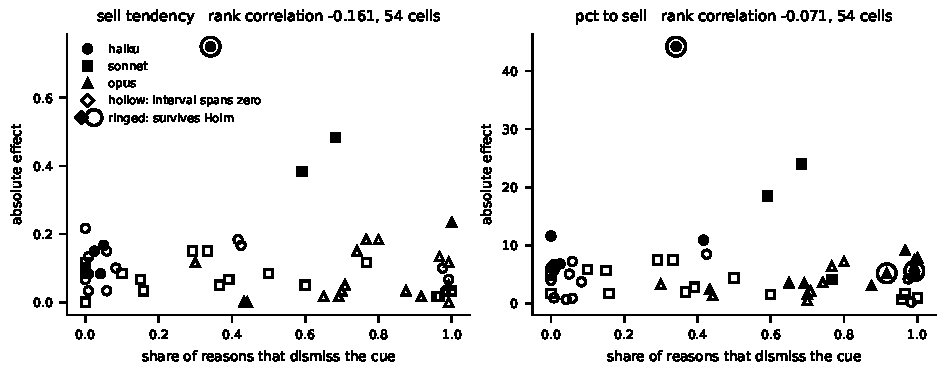
\includegraphics[width=\textwidth]{../figures/fig6_dissociation_acl.pdf}
  \caption{Dismissing the cue does not predict not acting on it. Each point
  is one model, effort and family cell: on the horizontal axis the share of
  that cell's one-sentence reasons that name the manipulated cue and discount
  it, on the vertical axis the size of that cell's effect, unsigned, because
  the claim is about magnitude. Only the six families the advisor ever refers
  to appear; the other three are never referred to at all, which the text
  takes up. If saying the right thing meant doing the right thing, the cloud
  would run downhill. The two Opus cells that survive Holm
  correction, at the right of the continuous panel, discount the cue in over
  nine tenths of their reasons and move with it anyway.}
  \label{fig:dissociation}
\end{figure*}
\else
\begin{figure}[t]
  \centering
  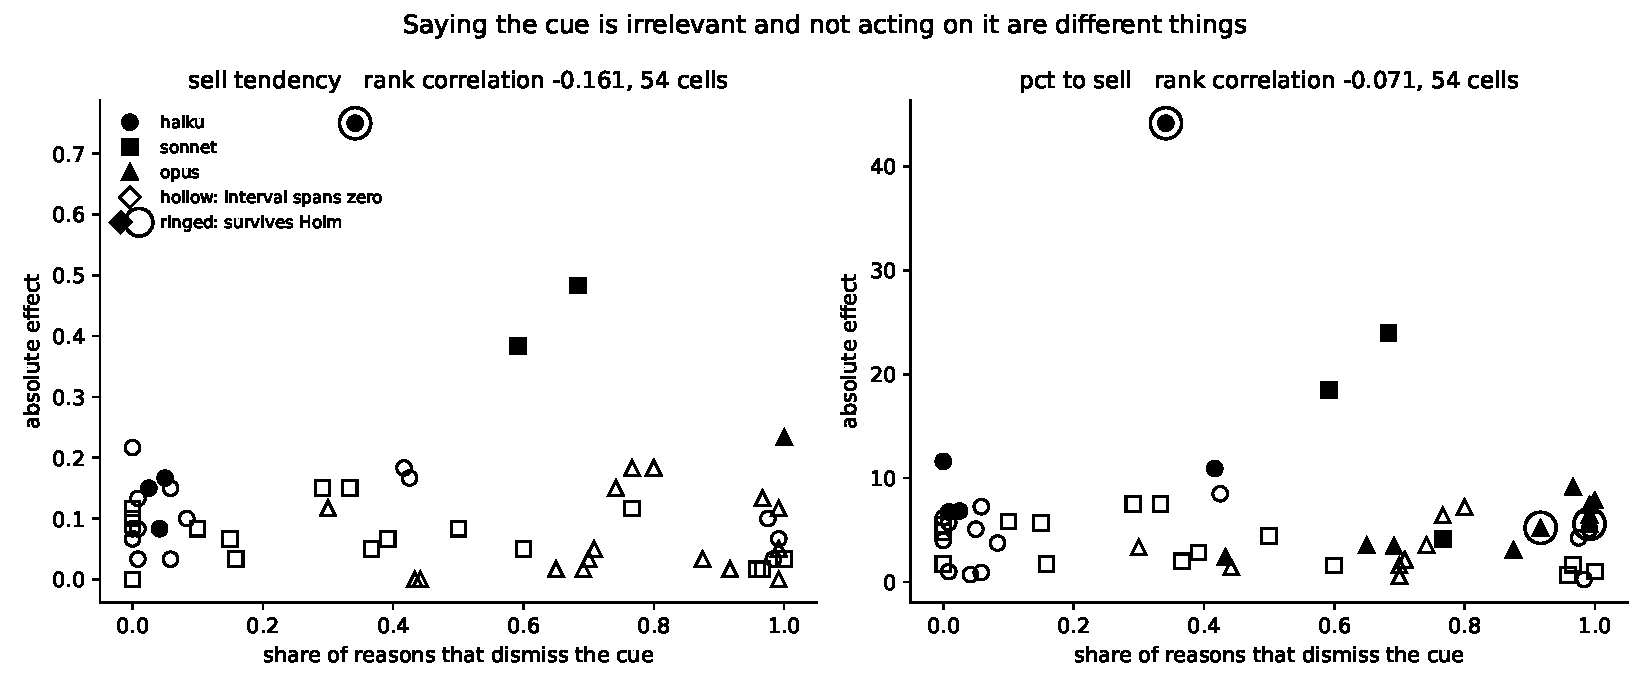
\includegraphics[width=\linewidth]{../figures/fig6_dissociation.pdf}
  \caption{Rejection rate against absolute effect, one point per model,
  effort and family cell, over the six families the advisor refers to. A flat
  cloud is the finding: the cells that discount the cue most are not the
  cells that move least.}
  \label{fig:dissociation}
\end{figure}
\fi


\paragraph{The dissociation.} Set the rejection rate of each cell against the
effect measured in that same cell, as Figure~\ref{fig:dissociation} does. If stated reasoning guarded against the
bias, a cell that discounts the cue in almost every reason it writes would
not move with it. Such cells exist, and they include the strongest results in
the study. Of 24 of 108 cells that discount the cue in at least 90\% of their
reasons, 7 of 24 still show an effect whose bootstrap interval excludes zero,
and 2 of 7 survive Holm correction across the whole family of tests. The two
that survive are Opus at \texttt{high} on anchoring, which discounts the
purchase price in 0.99 of its reasons and still shifts the recommended sale
by $+5.58$ percentage points \mbox{[$+2.83$, $+9.33$]}, $p_{\mathrm{Holm}} =
0.0189$; and Opus at \texttt{high} on mental accounting, which discounts the
accounting split in 0.92 of its reasons and still shifts it by $+5.22$
\mbox{[$+2.17$, $+8.97$]}, $p_{\mathrm{Holm}} = 0.0408$.

Only four cells in the entire study survive Holm correction, and they sit at
opposite ends of this scale. Two are the Opus cells above. The other two are
Haiku at \texttt{low} on disposition, on both measures, $p_{\mathrm{Holm}} =
0.0063$, a cell that discounts the cue in 0.34 of its reasons, the lowest
rate of any disposition cell in the design. The largest and most robust
effects in the study occur both where the model argues hardest against the
cue and where it argues least. For contrast, of the 30 of 108 cells that
essentially never name the cue, 6 of 30 show an effect clear of zero, which
is a similar share. Across all 54 nameable cells the rank correlation between
rejection rate and absolute effect is $-0.161$ on the categorical measure and
$-0.071$ on the continuous one: nothing, and if anything the wrong way. The
figure is the argument. A reader looking for the downhill cloud that stated
reasoning would produce will not find one.

\paragraph{What this does and does not establish.} The effort-to-rejection
result is identified, because the reasoning budget is set before the item is
seen. The rejection-to-bias association is not, and it fails for exactly the
reason this paper gives for declining to read Bini et al.'s self-reported
reasoning indicator as a treatment: the sentence and the recommendation are
produced in one forward pass, so neither is prior to the other and a third
property of the item can move both. What the dissociation supports is
narrower and still worth having. The explanation a model offers is not a
usable signal of whether that model was biased, because the cells where the
explanation most firmly rejects the cue are among the cells where the
behaviour most clearly follows it. An audit that reads the advisor's
reasoning and finds the right words in it has established that the right
words were produced.
